% This must be in the first 5 lines to tell arXiv to use pdfLaTeX, which is strongly recommended.
% \pdfoutput=1
% In particular, the hyperref package requires pdfLaTeX to break URLs across lines.

\documentclass[11pt]{article}

% Reduce space between paragraphs globally
\setlength{\parskip}{0pt}  % No space between paragraphs

% Reduce space between lines of text
\setlength{\baselineskip}{11pt} 



% Change "review" to "final" to generate the final (sometimes called camera-ready) version.
% Change to "preprint" to generate a non-anonymous version with page numbers.
\usepackage[review]{acl}

% Standard package includes
\usepackage{times}
\usepackage{amsmath}
\usepackage{latexsym}

\usepackage{fontspec}
\usepackage{polyglossia}
\setdefaultlanguage{english}
\setotherlanguage{urdu}
% \settextfont{Noto Nastaliq Urdu}
\usepackage{listings}
\usepackage{xcolor}
\usepackage{booktabs,tabularx}
\usepackage{appendix} % For appendix management

% Define Urdu font (you must have one of these installed)
\newfontfamily\urdufont[Script=Arabic]{Noto Nastaliq Urdu}
% For Vietnamese characters
% \usepackage[T5]{fontenc}
% See https://www.latex-project.org/help/documentation/encguide.pdf for other character sets

% This assumes your files are encoded as UTF-8
\usepackage[utf8]{inputenc}

% This is not strictly necessary, and may be commented out,
% but it will improve the layout of the manuscript,
% and will typically save some space.
\usepackage{microtype}

% This is also not strictly necessary, and may be commented out.
% However, it will improve the aesthetics of text in
% the typewriter font.
\usepackage{inconsolata}

%Including images in your LaTeX document requires adding
%additional package(s)
\usepackage{graphicx}

\usepackage{float}
\usepackage{array}
\usepackage{ragged2e}
\usepackage{fontspec}
\usepackage{polyglossia}
\usepackage{minted}
\setmainlanguage{english}
\setotherlanguage{urdu}
% \newfontfamily\urdufont[Script=Arabic,Language=Urdu]{Amiri}


% If the title and author information do not fit in the area allocated, uncomment the following
%
\setlength\titlebox{4cm}
\usepackage{titlesec}
\titleformat{\section}
  {\normalfont\normalsize\bfseries}  % <- No small caps or spacing
  {\thesection}{1em}{}

\titleformat{\subsection}
  {\normalfont\normalsize\bfseries}
  {\thesubsection}{1em}{}

% Reduce spacing before and after section titles
\titlespacing*{\section}
  {0pt}{0.3em plus 0.05em minus 0.05em}{0.2em plus 0.05em minus 0.05em}

\titlespacing*{\subsection}
  {0pt}{0.3em plus 0.05em minus 0.05em}{0.2em plus 0.05em minus 0.05em}

\titlespacing*{\subsubsection}
  {0pt}{0.3em plus 0.05em minus 0.05em}{0.2em plus 0.05em minus 0.05em}

%
% and set <dim> to something 5cm or larger.
\setlength{\parskip}{0.3em} % Space between paragraphs
\setlength{\parindent}{0pt} % Optional: remove indent

\renewcommand{\baselinestretch}{0.95}
\title{Corpora Generation for Urdu Grammatical Error Correction}

% Author information can be set in various styles:
% For several authors from the same institution:
% \author{Author 1 \and ... \and Author n \\
%         Address line \\ ... \\ Address line}
% if the names do not fit well on one line, use
%         Author 1 \\ {\bf Author 2} \\ ... \\ {\bf Author n} \\
% For authors from different institutions:
% \author{Author 1 \\ Address line \\  ... \\ Address line
%         \And  ... \And
%         Author n \\ Address line \\ ... \\ Address line}
% To start a separate ``row'' of authors use \AND, as in
% \author{Author 1 \\ Address line \\  ... \\ Address line
%         \AND
%         Author 2 \\ Address line \\ ... \\ Address line \And
%         Author 3 \\ Address line \\ ... \\ Address line}

\author{
    Syed Ahad, Burhanuddin Ezzi, Arsalan Hussain, Sandesh Kumar, Abdul Samad \\
    Habib University, Karachi, Pakistan \\
    \texttt{\{sa07753, be07724, mh07607\}@st.habib.edu.pk}, \texttt{\{sandesh.kumar, abdul.samad\}@sse.habib.edu.pk}
}

%\author{
%  \textbf{First Author\textsuperscript{1}},
%  \textbf{Second Author\textsuperscript{1,2}},
%  \textbf{Third T. Author\textsuperscript{1}},
%  \textbf{Fourth Author\textsuperscript{1}},
%\\
%  \textbf{Fifth Author\textsuperscript{1,2}},
%  \textbf{Sixth Author\textsuperscript{1}},
%  \textbf{Seventh Author\textsuperscript{1}},
%  \textbf{Eighth Author \textsuperscript{1,2,3,4}},
%\\
%  \textbf{Ninth Author\textsuperscript{1}},
%  \textbf{Tenth Author\textsuperscript{1}},
%  \textbf{Eleventh E. Author\textsuperscript{1,2,3,4,5}},
%  \textbf{Twelfth Author\textsuperscript{1}},
%\\
%  \textbf{Thirteenth Author\textsuperscript{3}},
%  \textbf{Fourteenth F. Author\textsuperscript{2,4}},
%  \textbf{Fifteenth Author\textsuperscript{1}},
%  \textbf{Sixteenth Author\textsuperscript{1}},
%\\
%  \textbf{Seventeenth S. Author\textsuperscript{4,5}},
%  \textbf{Eighteenth Author\textsuperscript{3,4}},
%  \textbf{Nineteenth N. Author\textsuperscript{2,5}},
%  \textbf{Twentieth Author\textsuperscript{1}}
%\\
%\\
%  \textsuperscript{1}Affiliation 1,
%  \textsuperscript{2}Affiliation 2,
%  \textsuperscript{3}Affiliation 3,
%  \textsuperscript{4}Affiliation 4,
%  \textsuperscript{5}Affiliation 5
%\\
%  \small{
%    \textbf{Correspondence:} \href{mailto:email@domain}{email@domain}
%  }
%}

\begin{document}
\maketitle
\begin{abstract}
Grammatical Error Correction (GEC) for Urdu remains an under-researched area due to the lack of annotated datasets. This paper addresses the challenge of generating a robust corpus for fine-tuning deep learning models aimed at Urdu GEC. We propose a method for synthesizing a large dataset by collecting errors from the Urdu WikiEdits history, learning from them, and inserting similar errors in grammatically correct sentences to generate incorrect sentences with grammatical errors, hence creating a pair of grammatically correct and incorrect sentences. Furthermore, we have created a Gold Dataset by extracting errors from exam copies of students. After the generation of the dataset, we have also fine-tuned various models against synthetically generated data and evaluated them against gold data to show the quality of synthetic data generation.
\end{abstract}

% \section{Introduction}

% Urdu is a language with a rich heritage and a script influenced by Persian, Arabic, Hindi, Sanskrit, and Turkish. It is widely spoken in South Asian countries, including Pakistan and India, by a large population. Despite its complexity and the variety of grammatical components, unfortunately, there has been little work done in the field of Urdu grammatical error correction (GEC). An automated GEC system for Urdu would greatly enhance content creation, digital communication tools, and educational platforms. To build a state-of-the-art model that generalizes well to a wide range of human grammatical errors and outputs correct sentences for grammatically incorrect inputs, we need a large corpus of training data.
% \\
% Although there isn't a vast corpus available for this task, there are proven methods (used for other languages) that can help generate such datasets. Our research mainly aims to investigate these techniques and apply them to the Urdu language to create a robust corpus of Urdu.

% In our research, we are tackling two primary research questions: (1) “Generation of synthetic datasets for a low-resource language like Urdu,” and (2) "Building a state-of-the-art model that can output correct sentences for input sentences that are grammatically incorrect but require a single edit (insertion, deletion, or substitution) of words for correction". 

% \section{Related Work}

% \citet{hindi} generates a parallel corpus of synthetic errors by inserting errors into grammatically correct sentences using a rule-based process, focusing specifically on inflectional errors. They generate this artificial dataset for fine-tuning of models, and for evaluating those models, they scrape the edit history of Wikipedia and use that as a real-world data source to test the fine-tuned model on. This paper encourages that their strategies for Hindi can be applied to other Indic fusional languages such as Urdu, Bengali, etc.

% \citet{jared} provides a strategy for corpora generation that uses the Wiki edits dataset, which benefits from a more accurate distribution of natural grammatical errors made by humans. In their research, errors are introduced probabilistically in the source sequences, randomly selecting deletion, insertion, replacement, or transposition of adjacent characters for each introduced error. The second approach they use for data generation is of round-trip machine translation through a high-resource bridge language. They further augment this data with the common errors found in the Wiki edit approach and introduce them in the dataset. The authors pre-train the model on the above Wikipedia revision dataset and then fine-tune the model on a Lang-8 dataset, which is a parallel corpus for GEC but with high noise. Wikipedia-derived data demonstrated to benefit significantly from finetuning on Lang-8 because the Wikipedia revision dataset contains corrections that are outside the scope of GEC.

% \citeposs{jennifer} paper introduces GenERRate, a probabilistic error-infliction tool that generates errors such as POS insertions, deletions, and substitutions. It performs well in some scenarios but has limitations, particularly in handling covert errors like sentence structure improvements. This synthetic data shows improved accuracy and recall, especially useful for small-to-medium corpora. Combining natural and synthetic data helps mitigate performance degradation, showing promise for augmenting training sets with artificial data. 
\section{Introduction}

The field of Grammatical Error Correction (GEC) has witnessed a paradigm shift in recent years, moving from early rule-based and statistical classifiers to deep learning approaches. Specifically, treating GEC as a sequence-to-sequence (Seq2Seq) translation task has become the standard in the field, largely following the pioneering work of \citet{yuan-2016}, who demonstrated the efficacy of Neural Machine Translation (NMT) architectures for correcting grammatical errors. However, the success of these supervised deep learning models is heavily contingent on the availability of massive, high-quality parallel corpora of grammatically incorrect and correct sentence pairs. While such resources exist for high-resource languages like English, they are virtually nonexistent for low-resource languages, creating a significant bottleneck for development.

Urdu is a language with a rich heritage and a script influenced by Persian, Arabic, Hindi, Sanskrit, and Turkish. (\cite{ButtAhmed2011}, \cite{Mangrio2016Loanwords}) It is widely spoken in South Asian countries, including Pakistan and India, by a large population. Despite its complexity and the variety of grammatical components, unfortunately, there has been little work done in the field of Urdu GEC. An automated GEC system for Urdu would greatly enhance content creation, digital communication tools, and educational platforms. To build a state-of-the-art model that generalizes well to a wide range of human grammatical errors and outputs correct sentences for grammatically incorrect inputs, we need a large corpus of training data.

To address this data scarcity, this paper proposes a robust method for synthetic data generation. We propose a pipeline that mines naturally occurring error patterns from Urdu Wikipedia revision histories and re-inflicts them onto clean text. In doing so, we tackle two primary research questions: (1) “Generation of synthetic datasets for a low-resource language like Urdu,” and (2) “Building a state-of-the-art model that can output correct sentences for input sentences that are grammatically incorrect.”

Finally, given the substantial morphosyntactic similarities Urdu shares with other Indo-Aryan languages such as Hindi, Punjabi, and Sindhi \citep{ButtAhmed2011, Mangrio2021MorphoPhonological}, we hypothesize that our data generation pipeline is transferable to this broader linguistic family. Provided that prerequisite resources such as reliable POS taggers and dependency treebanks are available, this methodology can be effectively adapted to develop robust GEC systems for other low-resource Indic languages.

\section{Related Work}

Research in GEC has largely focused on methods to overcome the scarcity of annotated training data through synthetic error generation \cite{bryant-etal-2023-grammatical}. This section outlines the evolution of these techniques from random noise injection to linguistically grounded probabilistic modeling.

\subsection{The Shift to Neural GEC and Data Scarcity}
As established by \citet{yuan-2016}, modeling GEC as a monolingual machine translation task allows for powerful generalization, provided sufficient parallel data exists. In the absence of large annotated corpora (such as NUCLE or Lang-8 used for English), researchers have turned to synthetic data generation. Early approaches, such as GenERRate by \citet{jennifer}, introduced probabilistic error-infliction tools to generate errors like POS insertions, deletions, and substitutions. While useful for small-to-medium corpora, purely random or simple rule-based noise often fails to capture the complexity of human errors, leading to models that do not generalize well to real-world inputs.

\subsection{Linguistically Grounded Error Generation}
To improve the quality of synthetic data, recent work has emphasized the importance of linguistic context over random noise. \citet{sidorov-2013} argued that traditional lexical n-grams are insufficient for modeling syntactic relations and demonstrated that Syntactic N-grams (utilizing POS tags) significantly improve error detection and correction. This theoretical foundation supports the move toward "kernel-based" or pattern-based error generation.

Building on this, \citet{ma-2022} utilized a Linguistic Rules-Based Generation (CLG) approach. They explicitly defined grammatical rules (e.g., "Structural Confusion") to generate synthetic errors that mimic the structural complexity of real mistakes. Their findings highlight that synthetically generated errors must be linguistically plausible to be effective for training NMT systems. This contrasts with earlier methods by \citet{jennifer}, which relied on hard-coded rules, by demonstrating that preserving the "grammatical severity" of an error is crucial for downstream model performance.

\subsection{Mining Error Distributions from Natural Data}
Rather than manually crafting linguistic rules, modern approaches attempt to learn error distributions directly from noisy data. \citet{felice-yuan-2014} were among the first to move away from inserting random errors, instead calculating conditional probabilities of errors based on linguistic context (e.g., $P(\text{error} | \text{POS tag})$) derived from learner corpora. Similarly, \citet{kasewa-2018} argued against random noise injection, proposing a method to learn the probability distribution of errors from a seed corpus and project that distribution onto clean text. This "mining and grafting" strategy ensures that the synthetic data reflects the natural distribution of errors made by humans, a technique we adopt in our pipeline by downsampling synthetic data to match natural error frequencies.

\subsection{GEC for Low-Resource and Indic Languages}
In the context of utilizing web-scale resources, \citet{jared} proposed generating corpora using Wikipedia edit histories (WikiEdits). They employed a dual strategy of probabilistic error introduction and Round-Trip Translation (RTT) through a high-resource bridge language. Their work demonstrated that Wikipedia revision histories contain valuable "natural" errors that benefit models significantly when fine-tuned.

Specific to Indic languages, \citet{hindi} adapted these strategies for Hindi, a language linguistically similar to Urdu. They generated a parallel corpus of synthetic errors by focusing on inflectional errors via a rule-based process and validated their models against scraped Wikipedia edit histories. Our work extends these methodologies to Urdu; however, rather than relying solely on rule-based inflection or random noise, we employ a kernel-based extraction method inspired by the syntactic dependencies highlighted by \citet{sidorov-2013} and the probabilistic mining approaches of \citet{felice-yuan-2014}, ensuring our synthetic corpus captures the specific morpho-syntactic nuances of Urdu.

\section{Dataset Generation}
\subsection{Methodology for Synthetically Generated Dataset}
\label{sec:Methodology_of_Dataset_Generation}

Our approach for creating a synthetically generated dataset is a pipeline that uses the established paradigm of "error annotation and infliction," a principled approach for creating synthetic data in low-resource settings \citep{alrehili2025developmentbalancedsyntheticdata}. In the first phase of our pipeline (Annotation Phase), given a set of correct and grammatically incorrect sentence pairs, learns the different types of errors from those pairs, and in its second phase (Infliction Phase), given clean Urdu sentences, outputs corrupted sentences resulting in GEC pairs, where the corruption is the same as the one learned from the set of correct and grammatically incorrect sentence pairs.

\subsubsection{Extraction of Errors from Wikipedia Revision Histories}
\label{sec:clean_wikiedits}
To capture natural grammatical errors for the Annotation phase, we mined Urdu Wikipedia revision histories, adopting the strategy used by \citet{hindi} for Hindi. Given that Wikipedia content in low-resource languages often originates from translation followed by human post-editing, the edit history provides a rich source of grammatical corrections. We extracted edit sequences, treating the final revision as the grammatically correct reference and the penultimate revision as the incorrect source. Following extraction, we applied a standard cleaning pipeline to filter noise, the details of which are provided in Appendix \ref{sec:Raw_Wiki-Edits_Cleaning}, which is also based on \cite{hindi}, ensuring that the errors collected are grammatical only. This process yielded the \textbf{Wiki-Edits Dataset}, comprising approximately 240,000 parallel sentence pairs.

\subsubsection{Error Annotation}
The goal of the annotation phase is to build a structured, context-rich database of observed grammatical errors from the \textbf{Cleaned Wiki-Edits Dataset} using each of its incorrect-correct sentence pairs.

First, we performed context-aware analysis using \textbf{Stanza} \cite{qi2020stanza} to extract POS tags, lemmas (root words), and morphological features for every word in each sentence pair in the \textbf{Cleaned Wiki-Edits Dataset}. Stanza was selected for its high accuracy on Urdu (Appendix \ref{Linguistic_Resources}). To ensure that our pipeline focuses on morphological shifts rather than spelling corrections, we established a closed vocabulary for Out-of-Vocabulary (OOV) checks derived from the UD 2.12 treebank \cite{bhathindi, palmer2009hindi}. This ensures tokenization consistency, as Stanza and our vocabulary share the same underlying schema from the treebank.

Next, we identified the precise edits transforming incorrect sentences into correct ones using a custom alignment algorithm inspired by \textbf{ERRANT} \citep{errant}, which classifies edits as ‘Insertion’ (I), ‘Deletion’ (D), or ‘Substitution’ (S); Figure~\ref{fig:alignment-example} shows an example. Unlike standard Levenshtein distance, our algorithm employs a linguistically motivated cost function to better model grammatical similarity (exact formulation in Appendix   \ref{sec:Alignment_Cost_Function}).
\vspace{5}
\begin{figure}
    \centering
    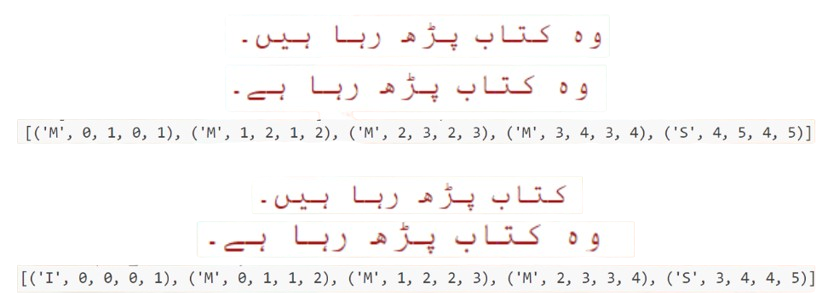
\includegraphics[width=0.5\textwidth]{alignment-example.png}
    \caption{Two example outputs of the alignment algorithm on the same grammatically incorrect input sentence (the top one in both examples), which has five words in it; "\texturdu{وہ}", "\texturdu{کتاب}", "\texturdu{پڑھ}", "\texturdu{رہا}", and "\texturdu{ہیں}". The output of the first example (transition of type S) shows that the sentence has 5 words in total, 4 matching words "M", and 1 substituted word "S". The output of the second example (transition of type S and I) shows that there has been an insertion "I" at the first index and a substitution at the last index.}
    \label{fig:alignment-example}
\end{figure}
\vspace{-0.5cm}

\paragraph{Kernel-Based Error Representation.}
To capture the grammatical environment of an error, we define a local context window, or "kernel," of size $k$. This consists of the token at the edit index ($w_i$) and its surrounding neighbors. For example, if $k=3$, the kernel includes the immediate left and right neighbors ($w_{i-1}, w_{i+1}$). We treat $k$ as a tunable hyperparameter to balance context-awareness against data sparsity. Rather than storing raw lexical forms, we abstract tokens into their \textbf{Morpho-Syntactic States} using Stanza.
    We observed that different error types require different levels of contextual granularity. Therefore, we defined distinct matching criteria for each operation:
\begin{itemize}
\setlength{\itemsep}{0pt}
\setlength{\parskip}{0pt}
    \item \textbf{Substitution Patterns:} We model this as a \textit{Morphological Transition} of the target word constrained by a \textit{Syntactic Frame}. The frame is defined strictly by the UPOS tags of the context window. The transition is defined by the change in morphological features of the middle word (e.g., \texttt{Case: Nom} $\rightarrow$ \texttt{Case :cc}). We do not constrain the morphological features of the surrounding tokens in the window for substitutions, allowing the pattern to generalize across different neighbor inflections.
    
    \item \textbf{Insertion and Deletion Patterns:} Since these operations involve the presence or absence of a word, we enforce a stricter context validation: the kernel is defined by both the UPOS tags \textit{and} the exact morphological features of the surrounding words in the context window. For example, in the case of $k=3$, deleting a postposition requires checking that the preceding noun is in the specific morphological state (e.g., Oblique) that licensed that postposition.
\end{itemize}

\paragraph{Annotation Storage.}
We aggregate these patterns into a database of observed errors, where each entry stores the matching criteria (Context UPOS and/or Features) and the transformation rules required to reproduce the error. For \textbf{Substitutions}, we record the specific mismatch in morphological features between the incorrect and correct words (e.g., a shift in Case). For \textbf{Deletions}, we store the exact surface word to be removed. For \textbf{Insertions}, we record the strict morphological context of the neighbors that indicates a missing word. Detailed schema definitions for these annotation objects are listed in Appendix \ref{sec:Annotation_Schema}.

\subsubsection{Error Infliction}
\label{sec:Infliction}
In the final phase, we utilize the learned error patterns to corrupt the \textbf{Makhzan Corpus} \cite{makhzan}, a large collection of cleaned, grammatically correct corpus consisting of around 270,000 Urdu sentences.

The infliction process operates by sliding a window across every sentence in the clean text, analyzing every possible local context window of size $k$ with Stanza to extract UPOS tags and morphological features. A context window in the clean sentence is identified as a candidate for corruption if its local morpho-syntactic context exactly matches the \textit{target} (correct) side of an error pattern stored in our Annotations Database. 
\\
To ensure high-quality generation, we apply specific linguistic constraints for each error type:

\paragraph{Substitution Infliction (The Lemma Constraint).}
Blindly substituting words based solely on POS tags would likely result in semantic drift. To prevent this, we generate substitution errors only when two conditions are met:
\begin{enumerate}
\setlength{\itemsep}{0pt}
\setlength{\parskip}{0pt}
    \item The word in the clean corpus must have morphological features matching the \verb|correct_feats| of a retrieved error pattern.
    \item There must exist a derived form from the \textbf{lemma} of the clean word matching the \verb|incorrect_feats| of the pattern (verified via our \textbf{Lemma Dictionary}, see Appendix \ref{sec:Lemma_Dictionary_Construction}).
\end{enumerate}
These conditions ensure that the generated error is a valid morphological variant of the original word, preserving the sentence's semantic core.

\paragraph{Insertion and Deletion Infliction.}
For these operations, we apply the logic of "reversing the correction" with strict context validation (described in Appendix \ref{sec:Indel_Logic}):
\begin{itemize}
\setlength{\itemsep}{0pt}
\setlength{\parskip}{0pt}
    \item \textbf{Deletions:} To simulate a deletion error, we identify a context in the clean sentence that matches a learned \textit{Insertion} pattern. If the clean words match the full morphological profile of an inserted word and its neighbors, the middle word is removed to generate the erroneous sentence of the pair.
    \item \textbf{Insertions:} To simulate an insertion error, we look for a context matching a learned \textit{Deletion} pattern. If a sequence of clean words matches the context defined by a Deletion pattern (where the 'gap' represents the token to be inserted), we inject the missing word as stored in the annotation database to generate the erroneous sentence of the pair.
\end{itemize}

\subsection{Creation of the Gold Test Dataset}
\label{sec:Gold_Dataset}

While synthetic data is essential for training in low-resource settings, evaluating models solely on synthetic data often leads to inflated performance metrics that fail to reflect real-world generalization. To establish a rigorous, unbiased benchmark for Urdu GEC, we curated a high-quality \textbf{Gold Test Dataset} of naturally occurring errors.

\paragraph{Data Sources and Curation.}
We collaborated with local educational institutions to procure work from Urdu exam papers of students (Grade 8 and above). The selected schools were chosen so that the student demographic there comprises both L1 and L2 learners to add diversity. Additionally, we extracted exercises from Urdu grammar workbooks designed for error correction tasks.

\paragraph{Scope and Filtering.}
We used help from expert linguists to manually filter out purely orthographic errors (spelling mistakes) or stylistic fluency edits that did not violate grammatical rules. This resulted in a dataset of 1,613 high-quality parallel pairs.

\paragraph{Error Distribution Statistics.}
To provide transparency regarding the types of errors covered, we provide statistics of the Gold-Dataset using the standardized ERRANT-type metrics \cite{errant} to illustrate the distribution of error types. We group the errant type metrics into 5 categories detailed in Appendix \ref{sec:macro}.
Table \ref{tab:gold_stats} details the breakdown of error types. 
\begin{table}[h]
\centering
\small
\resizebox{\columnwidth}{!}{
\begin{tabular}{l | r r | l}
\toprule
\textbf{Error Category} & \textbf{Count} & \textbf{\%} & \textbf{Example (Incorrect $\to$ Correct)} \\
\midrule
Verb \& Aux & 1,131 & 33.2 & \texturdu{کرتا} $\to$ \texturdu{کرتی} (Gender/Number) \\
Noun \& Pron & 733 & 21.5 & \texturdu{لڑکا} $\to$ \texturdu{لڑکے} (Oblique Case) \\
Adpos & 560 & 16.4 & \texturdu{کا} $\to$ \texturdu{کی} (Genitive Agreement) \\
Mod \& Misc & 618 & 18.2 & \texturdu{اچھا} $\to$ \texturdu{اچھے} (Adj Agreement) \\
Ortho & 362 & 10.6 & \texturdu{مسلہ} $\to$ \texturdu{مسئلہ} (Spelling) \\
\midrule
\textbf{Total Edits} & \textbf{3,404} & \textbf{100.0} & \textbf{Avg. 2.1 Errors / Sentence} \\
\bottomrule
\end{tabular}
}
\caption{Distribution of error types in the Gold Test Set (1,600 sentences), grouped by macro-grammatical categories.}
\label{tab:gold_stats}
\end{table}

To foster reproducibility and further research in Urdu NLP, we intend to release the \textbf{Gold Test Corpus} (1,613 pairs). 
\\The Gold corpus is, to our knowledge, the first expert-annotated GEC benchmark for Urdu derived from diverse educational sources.

\paragraph{Evaluation Protocol.}
This dataset is treated exclusively as a \textbf{Held-Out Test Set}. It is never seen by the model during any training experiment. By fine-tuning on synthetic data and evaluating on this completely different distribution of human errors, we ensure that our reported metrics reflect genuine grammatical generalization rather than pattern memorization.

\section{Optimization of Synthetic Data Generation}
\label{sec:Optimization}

The methodology described in Section \ref{sec:Methodology_of_Dataset_Generation} allows for flexible generation of errors based on three configurable parameters:
\begin{enumerate}
    \item \textbf{Context Window Size ($k$):} Defines the granularity of the morpho-syntactic environment required to trigger an error injection.
    \item \textbf{Sampling Strategy:} Determines the probability distribution used to select which error pattern to inflict when multiple matching patterns exist.
    \item \textbf{Error Density:} Controls the number of distinct errors injected into a single sentence.
\end{enumerate}
To determine the optimal configuration for generating the final synthetic corpus, we conducted a series of ablation studies.

\subsection{Optimization Protocol and Metrics}
\label{sec:Opt_Protocol}
For these optimization experiments, we utilized the \textbf{mT0-large} (1.2B parameters) \cite{muennighoff2022crosslingual} model as a proxy. We fine-tuned the model on different synthetic variations and evaluated performance on our Gold Dataset. All ablation runs used identical hyperparameters (detailed in Appendix \ref{sec:Training_Hyperparameters}) to ensure that performance differences were solely attributable to data characteristics.

To quantify performance, we utilize established metrics \cite{yuan-2016} for Grammatical Error Correction:
\begin{itemize}
    \setlength{\itemsep}{0pt}
    \setlength{\parskip}{0pt}
    \item \textbf{MaxMatch ($M^2$):} We use the $M^2$ scorer \cite{dahlmeier-ng-2012-better} to report \textbf{Precision}, \textbf{Recall}, and \textbf{F$_{\textbf{0.5}}$}.
    \item \textbf{GLEU:} The Generalized Language Evaluation Understanding metric \cite{napoles2015gleu}, utilized to measure fluency and overlap with reference sentences.
\end{itemize}

\subsection{Ablation 1: Context Window Size ($k$)}
The kernel size $k$ dictates the granularity of the error context. While a larger $k$ theoretically captures longer-range dependencies, it increases data sparsity, as finding larger exact $n$-gram matches in a clean corpus becomes exponentially harder. 

We experimented with $k=3$ ($\pm 1$ neighbor), $k=5$ ($\pm 2$), and $k=7$ ($\pm 3$). For this experiment, we held the \textbf{Sampling Strategy (Natural)} and \textbf{Error Density (Single Edit)} constant.

\begin{table}[h]
\centering
\small
\resizebox{\columnwidth}{!}{
\begin{tabular}{l|c|cccc}
\hline
\textbf{Kernel} & \textbf{Pairs} & \textbf{P} & \textbf{R} & \textbf{F\textsubscript{0.5}} &  \textbf{GLEU} \\
\hline
$k=3$ ($\pm 1$) & 1,270,500 & \textbf{36.74} & \textbf{15.52} & \textbf{28.85} & \textbf{68.6} \\
$k=5$ ($\pm 2$) & 156,085 & 28.26 & 12.04 & 22.26  & 67.05 \\
$k=7$ ($\pm 3$) & 18,689 & 27.84 & 08.44 & 19.07 & 67.3 \\
\hline
\end{tabular}}
\caption{Impact of Kernel Size on GEC performance. Dataset size represents the number of sentences where a matching context was found in the clean corpus.}
\label{tab:ablation_kernel}
\end{table}

As shown in Table \ref{tab:ablation_kernel}, increasing the kernel size led to a linear degradation in performance. This is directly correlated with the massive reduction in yieldable data; $k=7$ produced only $\sim$1.5\% of the data volume compared to $k=3$. Consequently, we selected $k=3$ as the optimal trade-off between local context awareness and data availability.

\subsection{Ablation 2: Error Sampling Strategy}
Errors in the Wiki-Edits dataset follow a "Natural" long-tail distribution, where simple errors (e.g., adposition drops) are vastly more frequent than complex morphological shifts. We compared \textbf{Natural Sampling} against \textbf{Temperature Sampling} ($\tau=0.5$), which flattens the distribution to give rare error patterns higher representation. 

For this experiment, we held \textbf{Kernel ($k=3$)} and \textbf{Error Density (Single Edit)} constant. Crucially, to ensure a fair comparison, the dataset size for Temperature Sampling was deliberately constrained to match the Natural Sampling size ($\approx$ 1.27M sentences) using similar implementation to logic detailed in Appendix \ref{sec:random_noise}.

\begin{table}[h]
\centering
\small
\resizebox{\columnwidth}{!}{
\begin{tabular}{lcccc}
\hline
\textbf{Strategy} & \textbf{P} & \textbf{R} & \textbf{F\textsubscript{0.5}} & \textbf{GLEU}\\
\hline
Natural Sampling & 36.74 & \textbf{15.52} & 28.85 & 68.6 \\
Temperature Sampling & \textbf{40.50} & 15.00 & \textbf{30.22} & \textbf{69.08} \\
\hline
\end{tabular}}
\caption{Impact of Sampling Strategy. Both datasets contained $\approx$ 1.27M sentences.}
\label{tab:ablation_sampling}
\end{table}

Temperature sampling yielded a notable improvement in Precision and $F_{0.5}$ (Table \ref{tab:ablation_sampling}). By upsampling rarer morphological error patterns, the model learned to generalize better to diverse error types, rather than overfitting to high-frequency surface edits.

\subsection{Ablation 3: Error Density (Single vs. Multi-Edit)}
Real-world texts often contain multiple errors per sentence. To support \textbf{Multi-Edit} generation, we engineered our infliction pipeline to apply errors iteratively from \textbf{right-to-left} to preserve index integrity. We compared a dataset with exactly one error per sentence against one where the number of errors follows a normal distribution using mean and standard deviation derived from Gold statistics (inspired by \cite{grundkiewicz-etal-2019-neural}).

For this experiment, we held \textbf{Kernel ($k=3$)} and \textbf{Sampling Strategy (Temperature)} constant.

\begin{table}[h]
\centering
\small
\resizebox{\columnwidth}{!}{
\begin{tabular}{lcccc}
\hline
\textbf{Configuration} & \textbf{P} & \textbf{R} & \textbf{F\textsubscript{0.5}} & \textbf{GLEU}\\
\hline
Single Edit & \textbf{40.50} & \textbf{15.00} & \textbf{30.22} & \textbf{69.08} \\
Multi-Edit (Normal Dist.) & 30.61 & 09.76 & 21.45 & 67.6 \\
\hline
\end{tabular}}
\caption{Impact of Error Density on GEC performance.}
\label{tab:ablation_density}
\end{table}

Even though our Gold Test set contains a significant proportion of multi-edit sentences (827 multi-edit vs. 805 single-edit pairs), the Multi-Edit model performed worse (Table \ref{tab:ablation_density}). We hypothesize that this is due to \textbf{infliction intensity}: applying a normal distribution of errors to the relatively short sentences typical of our corpus often obscures the semantic context required for reconstruction. Facing such high noise levels during training, the model struggles to learn precise correction mappings, leading to a notable drop in Precision (from 40.50 to 30.61). Consequently, we utilized the \textbf{Single Edit} configuration for the final corpus.

\subsection{Resulting synthetic GEC Corpora}
\label{sec:Datasets}

Based on the optimization study, we generated our final synthetic training corpus using \textbf{Kernel $k=3$}, \textbf{Temperature Sampling}, and \textbf{Single Edit} injection of length 1.27 million sentence pairs.
\\
To foster reproducibility and further research in Urdu NLP, we intend to release the \textbf{Synthetic Training Corpus} (1.27M pairs).

\section{Main Experiments}
\label{sec:Main_Experiments}

\subsection{Baselines and Comparisons}
To validate the efficacy of our proposed \textbf{Wiki-Edit Inflection} pipeline, we compare it against three distinct baselines, which are regarded as state-of-the-art in synthetic error generation:

\begin{enumerate}
    \item \textbf{Zero-Shot Baseline:} The raw pre-trained model without any GEC-specific fine-tuning. This serves as a control to measure the model's inherent ability to rewrite text.
    \item \textbf{Random Noise Injection:} We adapted the noise generation strategy proposed by \citet{grundkiewicz-etal-2019-neural}. We generated a synthetic dataset of 1.27M sentence pairs by applying probabilistic edit operations (insertion, deletion, substitution, swap) to the clean Makhzan corpus. While maintaining the statistical error distribution of the original study, we utilized Levenshtein distance for word substitutions to account for the lack of Urdu spell-checking resources (see implementation details in Appendix \ref{sec:random_noise}). This tests whether our linguistically motivated "Kernels" provide value over stochastic noise.
    \item \textbf{Neural AEG (Back-Translation):} Back translation is a widely used data augmentation technique in NLP where monolingual target-language text is translated back into the source language to create synthetic parallel data, thereby improving model robustness and performance in low-resource or error-correction settings. This approach has been identified as an effective artificial data generation method in recent surveys of grammatical error correction and translation research \citet{bryant-etal-2023-grammatical}. Following \citet{koyama-etal-2021-comparison}, \citet{rei-etal-2017-artificial}, and \citet{htut-tetreault-2019-unbearable}, we trained a sequence-to-sequence model to generate errors. We fine-tuned an \textbf{mT0-large} model on the \textit{Correct $\rightarrow$ Incorrect} direction using the raw Wiki-Edits data and used it to corrupt the clean Makhzan corpus. Then, following \citet{xie-etal-2018-noising}, we generated five predictions for each sentence with varying noise to equalize the dataset size. This compares our rule-based linguistic inflection against a purely neural approach. Then we trained the correction model using the same hyperparameters (listed in Appendix \ref{sec:Training_Hyperparameters}) as all our other models. We did not use a generative model as used by \citet{luhtaru-etal-2024-err} for the purposes of a fair comparison. We hypothesize the low scores to be the result of non-grammatical edits unfiltered in raw Wiki-Edits data, whereas our approach intrinsically performs the required filtering.
 
    \item \textbf{Raw Wiki-Edits:} We fine-tune directly on the \textbf{Wiki-Edits Dataset}, comprising approximately 240,000 parallel sentence pairs \ref{sec:clean_wikiedits} to test if our synthetic amplification provides benefits over the natural source data.

       \begin{table}[h]
\centering
\small
\resizebox{\columnwidth}{!}{
\begin{tabular}{lcccc}
\hline
\textbf{Approach} & \textbf{P} & \textbf{R} & \textbf{F\textsubscript{0.5}} & \textbf{GLEU}\\
\hline
Zero-Shot & 21.52 & \textbf{25.08} & 22.15 & 45.28 \\
Random Noise & 27.70 & 09.24 & 19.79 & 67.62 \\
Neural AEG & 10.51 & 03.04 & 07.05 & 62.58 \\
Raw Wiki-Edits & 20.74 & 05.40 & 13.22 & 66.02 \\
Our Approach & \textbf{40.50} & 15.00 & \textbf{30.22} & \textbf{69.08} \\
\hline
\end{tabular}}
\caption{Our approach compared with baselines.}
\label{tab:ablation_density}
\end{table}

\end{enumerate}

\subsection{Models and Implementation}
We evaluated our finalized synthetic data on three competitive multilingual architectures to demonstrate model-agnostic gains:
\begin{itemize}
    \item \textbf{mT0-large} (1.2B parameters): An instruction-tuned variant of mT5.
    % \item \textbf{ByT5-base} (582M parameters): A token-free model operating on raw bytes, theoretically advantageous for morphological errors.
    \item \textbf{NLLB-3.3B}: A massive multilingual translation model.
\end{itemize}

All models were fine-tuned using the \textbf{Adafactor} optimizer. Specific hyperparameters for all experiments are detailed in Appendix \ref{sec:Training_Hyperparameters}. Results are reported using the metrics defined in Section \ref{sec:Opt_Protocol}.

\begin{table*}[!t]
\centering
\scriptsize
\caption{Category-wise F\textsubscript{0.5} and GLEU scores on the gold test set.}
\label{tab:category_results}

\setlength{\tabcolsep}{3pt}
\renewcommand{\arraystretch}{1.1}

\begin{tabular}{l l cc cc cc cc cc cc}
\toprule
 &  & 
 \multicolumn{10}{c}{\textbf{Error Categories}} \\
\cmidrule(lr){3-12}

\textbf{Model} & \textbf{Variant} &
\multicolumn{2}{c}{Verb \& Aux} &
\multicolumn{2}{c}{Noun \& Pron} &
\multicolumn{2}{c}{Adpos} &
\multicolumn{2}{c}{Mod \& Misc} &
\multicolumn{2}{c}{Ortho} &
\multicolumn{2}{c}{Overall} \\

\cmidrule(lr){3-4}
\cmidrule(lr){5-6}
\cmidrule(lr){7-8}
\cmidrule(lr){9-10}
\cmidrule(lr){11-12}
\cmidrule(lr){13-14}

 &  &
F\textsubscript{0.5} & GLEU &
F\textsubscript{0.5} & GLEU &
F\textsubscript{0.5} & GLEU &
F\textsubscript{0.5} & GLEU &
F\textsubscript{0.5} & GLEU &
F\textsubscript{0.5} & GLEU \\
\midrule


MT0 
    & large (baseline)
 & 24.27 & 45.35 & 16.35 & 43.71 & 27.10 & 51.21 & 22.20 & 47.74 & 13.44 & 36.20 & 22.15 & 45.28 \\    
    & large (finetuned)
 & 32.74 & 67.62 & 18.56 & 66.35 & 49.86 & 78.03 & 8.36 & 73.89 & 23.20 & 70.63 & 30.22 & 69.08 \\

\addlinespace

NLLB
     & 3.3B (baseline)
 & 7.12 & 23.29 & 3.88 & 23.07 & 11.05 & 23.33 & 11.38 & 22.72 & 2.07 & 30.19 & 7.00 & 23.51 \\
     & 3.3B (finetuned)
 & 29.86 & 66.04 & 16.84 & 62.83 & 37.68 & 74.48 & 14.29 & 71.73 & 13.01 & 66.43 & 26.12 & 66.66 \\

\bottomrule
\end{tabular}
\end{table*}


\section{Results and Analysis}
This section presents the empirical results of our experiments. 

\subsection{Main Quantitative Results}
To measure the impact of our synthetic corpus, we evaluated each model on the held-out Gold Dataset in two settings: a zero-shot baseline (before fine-tuning) and after fine-tuning on our 1.27 million sentence pairs. The results are summarized in Table~\ref {tab:category_results}.

The results in Table~\ref {tab:category_results} reveal a substantial and consistent improvement across all metrics for both models after being fine-tuned on our synthetic corpus. The low baseline scores, particularly for NLLB, confirm that even powerful multilingual models lack specialized GEC capacity for Urdu out-of-the-box. Fine-tuning provides a dramatic performance boost.
% --- CONCLUSION SECTION ---
\section{Conclusion}
\label{sec:conclusion}

This paper addressed the critical scarcity of resources for Urdu Grammatical Error Correction (GEC) by introducing a principled, two-phase pipeline for large-scale synthetic corpus generation. Our approach learns fine-grained, context-aware error patterns from Wikipedia revision histories and systematically inflicts them onto a clean monolingual corpus, resulting in two key contributions: a replicable generation methodology and the release of a 1.27 million-pair synthetic corpus and a "Gold" test set. The profound effectiveness of this approach is confirmed by our experiments, which show dramatic performance gains across state-of-the-art models like mT0 and NLLB after fine-tuning. These results validate our method and provide the essential contributions to spur the development of practical GEC tools for millions of Urdu speakers.
Furthermore, given the substantial morphosyntactic similarities Urdu shares with other Indo-Aryan languages such as Hindi, Punjabi, and Sindhi \citep{ButtAhmed2011, Mangrio2021MorphoPhonological}, we hypothesize that our data generation pipeline is transferable to this broader linguistic family. Provided that prerequisite resources such as reliable POS taggers and dependency treebanks are available, this methodology can be effectively adapted to develop robust GEC systems for other low-resource Indic languages.

% --- LIMITATIONS SECTION ---
\subsection{Limitations}
\label{sec:limitations}

While our work establishes a strong baseline, we acknowledge several limitations that offer avenues for future research:

\begin{itemize}
    \item \textbf{Source Data Domain:} Although the WikiEdits corpus provides a rich source of naturalistic errors, its encyclopedic style may not fully capture the nuances and error patterns common in other domains, such as conversational text or creative writing. The error distribution is primarily reflective of Wikipedia contributors, which may differ from that of language learners.

    \item \textbf{Scope of Error Correction:} Our kernel-based approach, which relies on a three-word local context, is highly effective for single-token edits (substitutions, insertions, deletions) but may not adequately capture more complex, non-local grammatical errors, such as incorrect sentence structure or discourse-level phenomena.

    \item \textbf{Evaluation on Limited Gold Data:} Due to the scarcity of annotated resources for Urdu, our "Gold" test set, while high-quality, is of a limited size. A larger, more diverse evaluation benchmark would be needed to make more definitive claims about real-world performance across different demographics of Urdu speakers.

    \item \textbf{Computational Constraints:} Fine-tuning large models required significant computational resources, which constrained our ability to conduct more extensive hyperparameter searches or train for extended epochs. This may have prevented some models from reaching their full potential on our dataset.
\end{itemize}

% --- ETHICAL STATEMENT SECTION ---
\section{Ethical Statement}
\label{sec:ethics}

We have considered the ethical implications of our work throughout the research process.

\begin{itemize}
    \item \textbf{Data Sources and Privacy:} The primary source for our synthetic data generation, Wikipedia, is a public resource with content licensed under Creative Commons (CC BY-SA 3.0). The text is encyclopedic and generally non-personal. While we did not implement an explicit PII removal step, a manual review of a sample of the data did not reveal any instances of sensitive personal information. The usernames associated with edits are pseudonymous and were not used in any part of our analysis. The "Gold Dataset" was derived from anonymized student exam papers, collected with institutional consent for research purposes. All personally identifiable information was removed during the manual extraction process.

    \item \textbf{Potential for Bias:} Our synthetic dataset inherits the biases present in its source corpora. The "Wiki-Edits Dataset" reflects the language and error patterns of its contributors, while the "Gold Dataset" reflects those of students in a specific educational context. The models trained on this data will consequently learn these biases. We believe that releasing both datasets allows future researchers to study and mitigate these biases, but users of models trained on this data should be aware of its origins.

    \item \textbf{Intended Use and Impact:} The intended use of our work is to advance NLP research and tool development for Urdu, a low-resource language. An automated GEC system has a significant positive impact by enhancing content creation, improving digital communication tools, and providing valuable feedback in educational platforms. We are not aware of any direct potential for malicious use of this technology. Both the code and the datasets will be made publicly available to ensure transparency, reproducibility, and to foster further research for the benefit of the Urdu-speaking community.
\end{itemize}



% Custom bibliography entries only
\bibliography{custom}

\clearpage

\begin{center}
    \textbf{\Large Appendices}
\end{center}
\noindent
\begin{appendices}
\section{Raw Wiki-Edits Cleaning}
\label{sec:Raw_Wiki-Edits_Cleaning}
To ensure the quality of the "Wiki-Edits Dataset," the raw data extracted from Wikipedia revision histories were subjected to the following cleaning pipeline:
\begin{enumerate}
\setlength{\itemsep}{0pt}  % Reduce the space between items
  \setlength{\itemsep}{0pt}
    \setlength{\parskip}{0pt}
    \item \textbf{Character Filtering:} Removal of extra whitespaces and non-Urdu characters (e.g., emojis or unsupported symbols).
    \item \textbf{Noise Filtering:} Removal of sequences containing a high percentage of numeric or non-alphabetical characters, as these usually represent metadata or formatting code rather than natural language.
    \item \textbf{Deduplication:} Removal of extremely similar sentence pairs to prevent data leakage and redundancy.
    \item \textbf{Unicode Normalization:} Translation of non-Urdu Unicode characters to the standard Urdu range (e.g., converting Arabic-specific Unicode points to their Urdu equivalents) and translation of English numerals to Urdu numerals using normalization provided by the UrduHack \cite{urduhack} Toolkit.
\end{enumerate}

\section{Linguistic Resources}
\label{Linguistic_Resources}
 Stanza's Urdu model, fine-tuned on the UD 2.12 treebank dataset \cite{bhathindi, palmer2009hindi}, demonstrates high performance, with reported accuracy scores of 94.78\% for lemmatization, 92.98\% for UPOS tagging, and 84.06\% for morphological features. This level of accuracy is crucial for the annotation phase, as it ensures that the grammatical context of each error is captured with high fidelity.

\section{Alignment Cost Function}
\label{sec:Alignment_Cost_Function}
Our alignment algorithm utilizes a weighted cost function to prioritize grammatical changes over semantic substitutions. The cost between an original token \(\texttt{o}\) and a corrected token \(\texttt{c}\) is calculated as:
\vspace{-0.25cm}
\[ \texttt{Cost}(\texttt{o}, \texttt{c}) = \texttt{Cost}_{\texttt{lemma}} + \texttt{Cost}_{\texttt{pos}} + \texttt{Cost}_{\texttt{char}} \]
\vspace{-0.25cm}
Where:
% \vspace{-0.1cm}
\begin{itemize}
\setlength{\itemsep}{0pt}  % Reduce the space between items
  \setlength{\parskip}{0pt}  % Adjust paragraph skip between items
  \setlength{\topsep}{0pt} 
    \item \textbf{\(\texttt{Cost}_{\texttt{lemma}}\)} is 0 if the lemmas are identical and 0.499 otherwise. This penalizes substitutions that change the base meaning of the word.\footnote{0.499 is chosen to be just below the threshold of 0.5 to prioritize lemma matches over POS mismatches in edge cases}
    \item \textbf{\(\texttt{Cost}_{\texttt{pos}}\)} is 0 if the Universal Part-of-Speech (UPOS) tags are the same, 0.25 if both are open-class POS tags (e.g., Noun to Verb), and 0.5 otherwise. This reflects the grammatical severity of the change.
    \item \textbf{\(\texttt{Cost}_{\texttt{char}}\)} is the normalized Indel distance between the token for minorcounting minor for spelling variations.
\end{itemize}
This cost function ensures that the alignment prefers linguistically plausible edits, such as changing an inflection, over substituting an unrelated word.

\section{Detailed Annotation Schema}
\label{sec:Annotation_Schema}

This appendix details the data structures used to implement the kernel-based error representation described in Section 3.1.2. The schema is designed to be flexible for any kernel size $k$, though we illustrate using the default $k=3$.

\subsection{Kernel Definition and Placeholders}
To handle boundary conditions, the "kernel" utilizes a specific placeholder tag, \verb|'%'|, to handle edge cases:

\begin{itemize}
\setlength{\itemsep}{0pt}
\setlength{\parskip}{0pt}
    \item \textbf{Standard Context:} For Substitution and Insertion errors, the kernel is a list of $k$ UPOS tags (e.g., \verb|[UPOS_left, UPOS_middle, UPOS_right]|). If the edit occurs at the start or end of a sentence, the missing neighbor is replaced with \verb|'%'|.
    \item \textbf{Deletion Context:} Since a Deletion error represents a "gap" between two words, the middle element is always the placeholder. The structure is strictly \verb|[UPOS_left, '%', UPOS_right]| (for $k=3$).
\end{itemize}

\subsection{JSON Annotation Objects}
For every observed edit, a structured JSON object is created. The specific fields vary by error type to optimize for the distinct context requirements of each operation (e.g., storing neighbor features for Indels but not for Substitutions).

\paragraph{Substitution (S)}
An annotation is created only if both the incorrect and correct words pass the OOV check.
\begin{itemize}
\setlength{\itemsep}{0pt}
\setlength{\parskip}{0pt}
    \item \verb|type|: 'S'
    \item \verb|kernel_upos|: The list of three UPOS tags forming the syntactic frame.
    \item \verb|incorrect_feats|: A \verb|UPOSFeats| object containing the UPOS and morphological features (e.g., \texttt{Gender=Masc|Number=Sing}) of the \textbf{source} word.
    \item \verb|correct_feats|: A \verb|UPOSFeats| object containing the features of the \textbf{target} word.
    \item \verb|occurrence|: A counter for this specific morphological transition under this kernel.
\end{itemize}

\paragraph{Deletion (D)}
An annotation is created if the deleted word and its neighbors pass the OOV checks. Note that, unlike Substitution, we store the morphological features of the \textit{neighbors} to ensure strict context matching.
\begin{itemize}
\setlength{\itemsep}{0pt}
\setlength{\parskip}{0pt}
    \item \verb|type|: 'D'
    \item \verb|kernel_upos|: The three-element kernel with \verb|'%'| in the middle.
    \item \verb|kernel_feats|: A list of \verb|UPOSFeats| objects for the left and right context neighbors.
    \item \verb|deleted_words|: The list containing the exact surface word that was deleted.
    \item \verb|occurrence|: Frequency counter.
\end{itemize}

\paragraph{Insertion (I)}
An annotation is created if the inserted word and the surrounding context in the correct sentence pass the OOV check.
\begin{itemize}
\setlength{\itemsep}{0pt}
\setlength{\parskip}{0pt}
    \item \verb|type|: 'I'
    \item \verb|kernel_upos|: The list of three UPOS tags.
    \item \verb|kernel_feats|: A list of \verb|UPOSFeats| objects for all three words (Left, Inserted, Right) to capture the full morphological agreement context.
    \item \verb|inserted_word|: The exact surface word that was inserted.
    \item \verb|occurrence|: Frequency counter.
\end{itemize}

\subsection{Storage Structure}
To allow for efficient querying during the infliction phase, these objects are stored in a dictionary keyed by the syntactic frame:
\begin{itemize}
    \item \textbf{Key:} The string representation of the \verb|kernel_upos| list (e.g., \verb|"['NOUN', '%', 'VERB']"|).
    \item \textbf{Value:} A list of all unique annotation objects (as defined above) that share that syntactic frame.
\end{itemize}

Figure \ref{fig:error_annotation} visualizes how these objects are serialized in the final JSON output.

\begin{figure}[h]
    \centering
    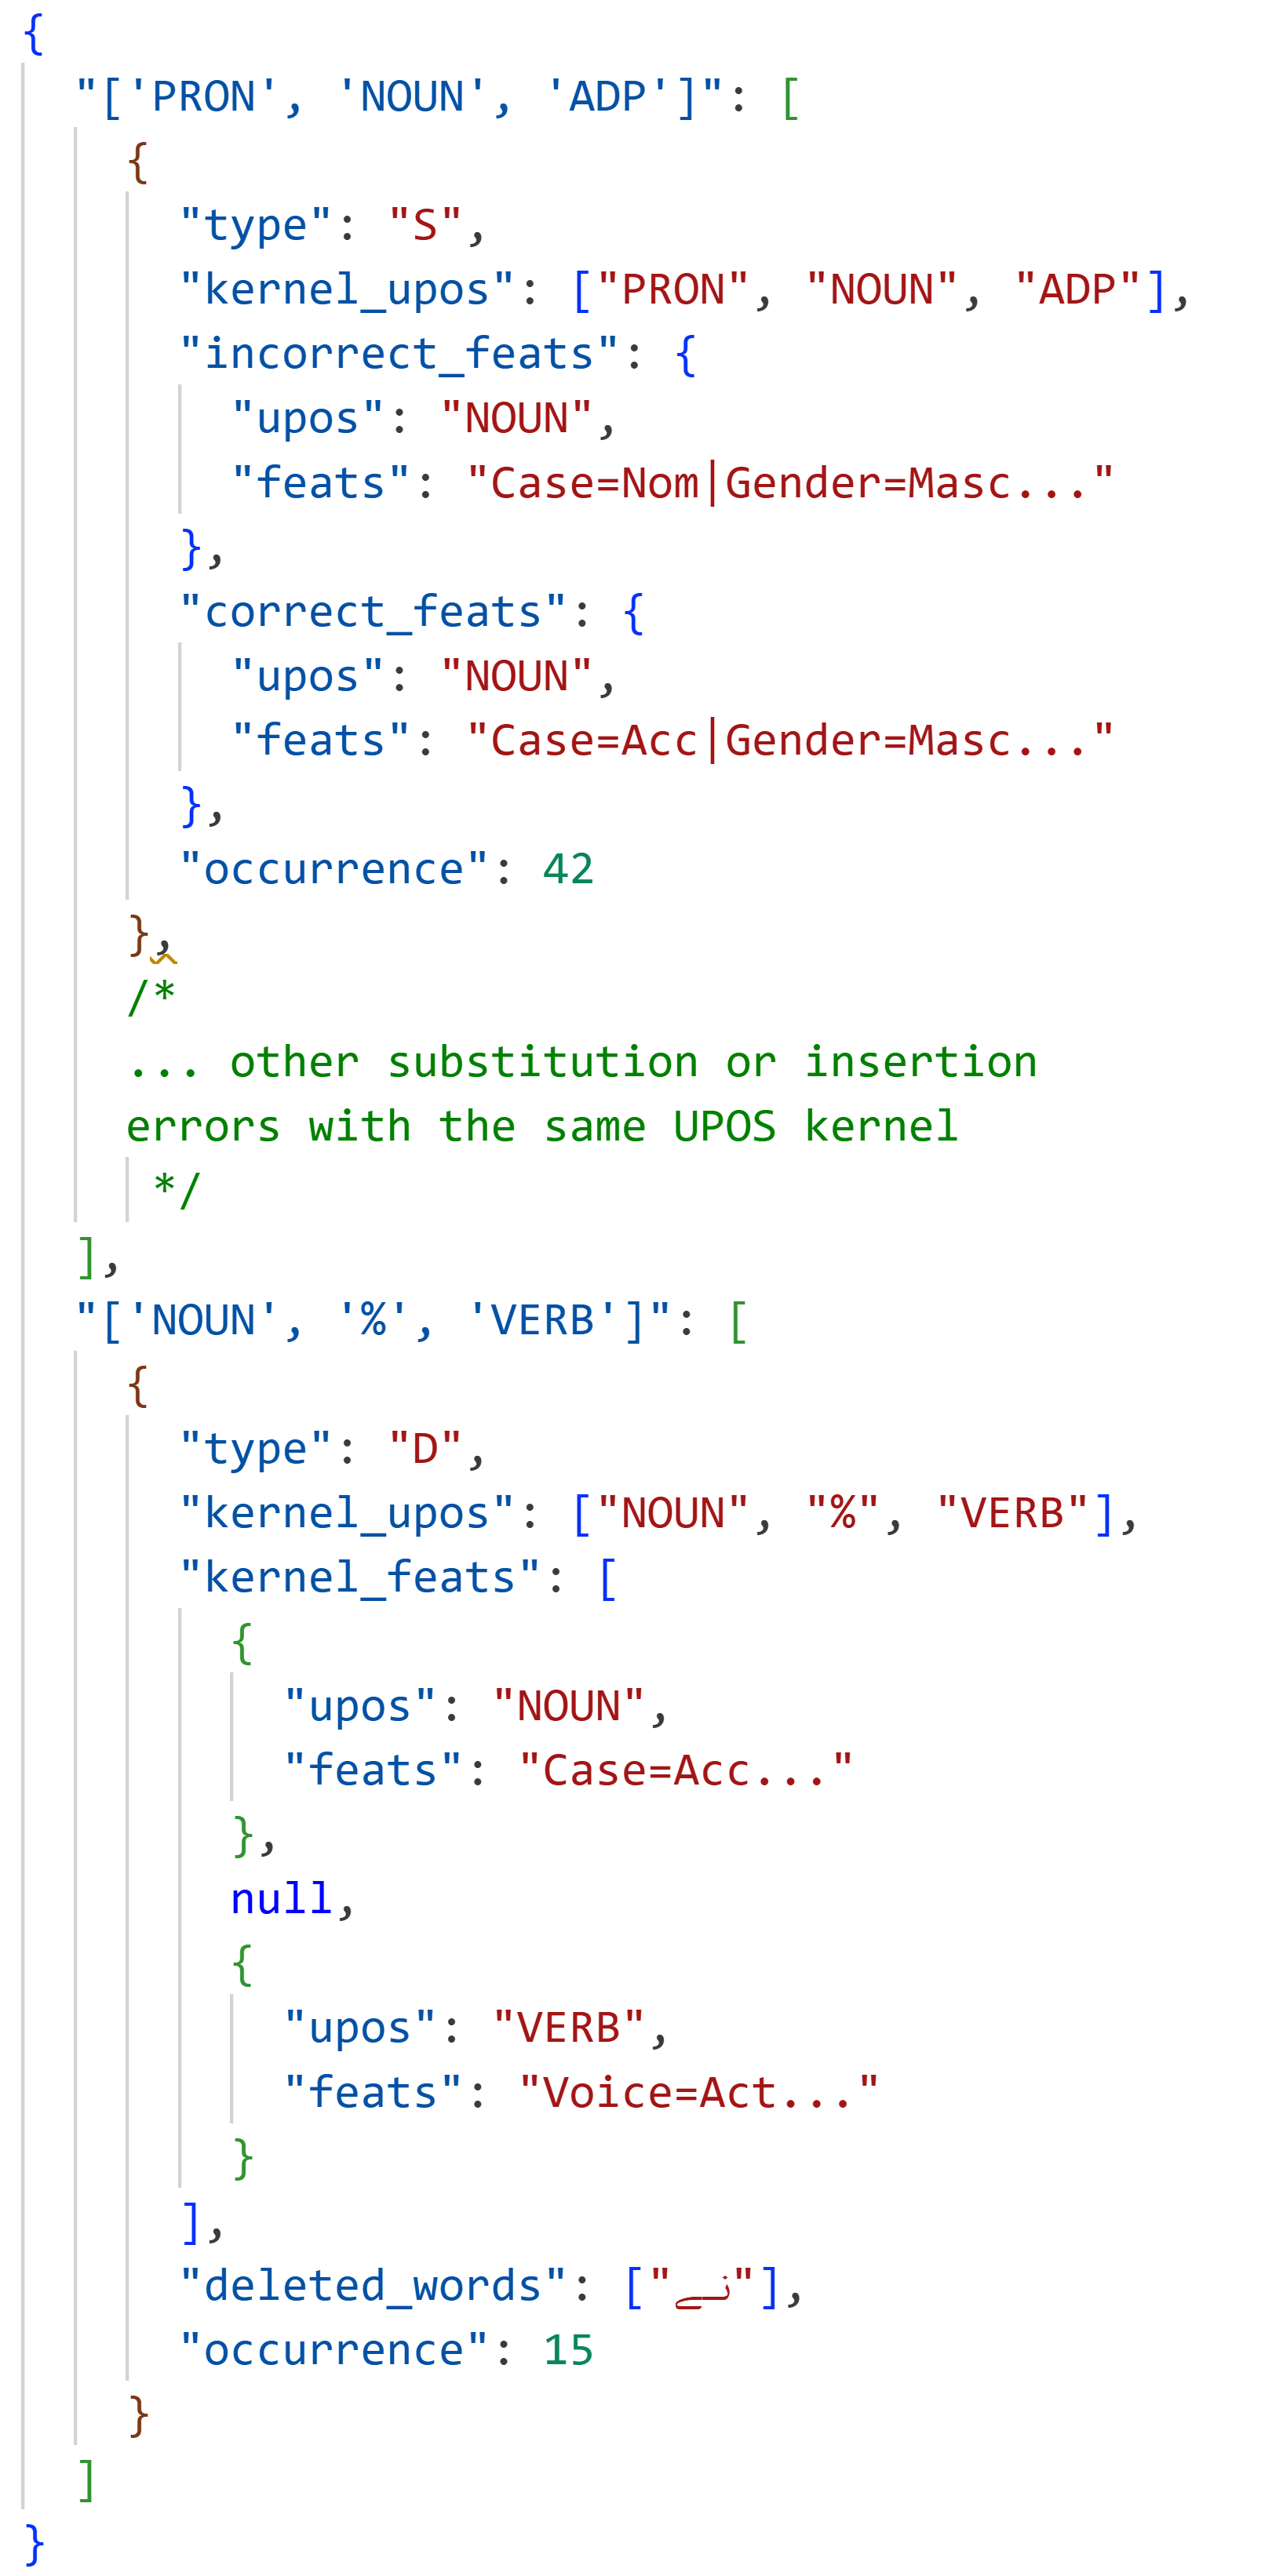
\includegraphics[width=0.5\textwidth]{2final.png}
    \caption{Example of the Final Annotation Data Structure showing a Substitution object (top) and a Deletion object (bottom).}
    \label{fig:error_annotation}
\end{figure}

\section{Infliction Mechanism Details}
\label{sec:Infliction_Details}

\subsection{Lemma Dictionary Construction}
\label{sec:Lemma_Dictionary_Construction}
To enable the \textbf{Lemma Constraint} described in  Section \ref{sec:Infliction}, we required a mapping that could answer the question: \textit{"For a given root lemma, what are all the valid morphological surface forms that exist in standard Urdu?"}

We constructed this knowledge base by iterating through every sentence in the \textbf{UD 2.12 Urdu Treebank} \cite{bhathindi, palmer2009hindi}. Since this treebank is manually annotated by linguists, it serves as a ground-truth source for valid morphological variation. The construction process was as follows:
\begin{enumerate}
    \item We iterated through all sentences in the treebank.
    \item For every token, we extracted its \textbf{Lemma}, its \textbf{Surface Form}, and its \textbf{Morphological Features} (e.g., \texttt{Case}, \texttt{Gender}, \texttt{Number}).
    \item We populated two dictionaries; One which stores all surface forms of a lemma, and two where the key is the \textit{word} which can be a lemma, or a surface form, and the value is a list of observed \textit{Feature Set}.
\end{enumerate}

Figure \ref{fig:lemma_structure} visualizes the first dictionary structure. Figure \ref{fig:lemma_lookup} shows the second diagram. Wenary structure; we use their combination in our infliction algorithm to dynamically generate the "incorrect" version of a word found in the clean corpus. For example, if the clean corpus contains the masculine verb form \textit{karta} (lemma: \textit{kar}), and the error pattern dictates a switch to feminine, we query the first dictionary to get the key \textit{kar} and query the second dictionary to retrieve the valid feminine form \textit{karti}, provided it was observed in the treebank with the required feature set.

\begin{figure}[H]
    \centering
    
\includegraphics[width=0.45\textwidth]{latex/lemma_new.PNG}
    \caption{Structure of the pre-compiled word-to-lemma dictionary. The lemma serves as the key, pointing to a list of all its derived forms observed in the treebank.}
    \label{fig:lemma_structure}
\end{figure}

\begin{figure}[H]
    \centering
    
\includegraphics[width=0.45\textwidth]{latex/lemma_lookup_copy.png}
    \caption{Example of the UD 2.12 treebank data represented as a dictionary. This is used during the Candidate Search phase to ensure that a target incorrect form corresponds to a valid grammatical usage.}
    \label{fig:lemma_lookup}
\end{figure}

\subsection{Insertion and Deletion Context Validation}
\label{sec:Indel_Logic}
While Substitutions rely on lemma lookups, Insertion and Deletion infliction relies on strict context matching. To ensure high fidelity:
\begin{itemize}
    \item \textbf{Pre-processing:} We apply character normalization to the clean text and run the Stanza pipeline to generate \verb|UPOSFeats| objects.
    \item \textbf{Sliding Window:} We utilize a sliding window of size $k$ (set to $k=3$ for our primary experiments). To optimize performance, we compute a hash of the $k$-gram UPOS tag sequence to instantly retrieve relevant error patterns from the Annotations Database.
    \item \textbf{OOV Safety:} Before any deletion or insertion is finalized, we perform an Out-of-Vocabulary (OOV) check on the target word. This prevents the system from learning or propagating typos or rare spellings that may have existed in the noisy Wikipedia source.
\end{itemize}

\section{Training Hyperparameters}
\label{sec:Training_Hyperparameters}

All neural models in this work were trained using a consistent set of hyperparameters to ensure fair comparison across experiments. These values were selected based on preliminary validation experiments and computational constraints.

\begin{table}[h]
\centering
\small
\setlength{\tabcolsep}{6pt}
\begin{tabular}{l c}
\hline
\textbf{Hyperparameter} & \textbf{Value} \\
\hline
Maximum sequence length & 128 \\
Batch size & 8 \\
Gradient accumulation steps & 4 \\
Effective batch size & 32 \\
Optimizer & Adafactor \\
Learning rate & $5 \times 10^{-6}$ \\
Number of epochs & 1 \\
Mixed precision & bfloat16 (bf16) \\
\hline
\end{tabular}
\caption{Training hyperparameters used for all model fine-tuning experiments.}
\label{tab:training_hyperparameters}
\end{table}

\section{Random Noise Implementation}
\label{sec:random_noise}
Our random noise baseline follows the statistical noise injection method described by \citet{grundkiewicz-etal-2019-neural}. We applied word-level and character-level noise to clean sentences with the following parameters:

\paragraph{Error Rates:} For each sentence, an error probability $p$ was sampled from a normal distribution $\mathcal{N}(\mu, \sigma)$. We set $\mu = 0.2$ based on the empirical error rate observed in our Gold Test Set, and $\sigma = 0.2$ following the reference study.

\paragraph{Operations:} Edits were applied based on the operation distribution: Substitution ($0.7$), Deletion ($0.1$), Insertion ($0.1$), and Swap ($0.1$). Furthermore, character-level noise (typos) was applied to $10\%$ of tokens.

\paragraph{Confusion Sets:} The reference study utilizes Aspell to generate confusion sets for word substitutions. Due to the lack of a robust phonetic spellchecker for Urdu, we generated confusion sets using Levenshtein Edit Distance. For any given word, candidates were selected from the vocabulary if they were within an edit distance of 2. In cases where no Levenshtein neighbors were found, the system fell back to random word substitution.

\section{Macro Error Categories}
\label{sec:macro}
For analysis and reporting, fine-grained ERRANT tags are grouped into linguistically motivated macro categories. Each macro category aggregates all operation types—Missing (M), Unnecessary (U), and Replacement (R)—for the listed tags.

\subsubsection{Verb & Auxiliaries}
This category covers the verbal complex, including tense, aspect, mood, and subject–verb agreement. It includes both root substitutions and inflectional changes affecting main verbs and auxiliary verbs.

ERRANT tags included:
\texttt{VERB}, \texttt{VERB:INFL}, \texttt{AUX}, \texttt{AUX:INFL}

\subsubsection{Nouns & Pronouns}
This category encompasses nominal entities and captures errors related to gender, number, and case, particularly the oblique form required before postpositions. Errors involving proper nouns are also included.

ERRANT tags included:
\texttt{NOUN}, \texttt{NOUN:INFL}, \texttt{PRON}, \texttt{PRON:INFL}, \texttt{PROPN}, \texttt{PROPN:INFL}

\subsubsection{Adpositions}
This category focuses on the Urdu adpositional system, including case markers such as \textit{ne} and \textit{ko}, as well as genitive agreement forms \textit{ka}, \textit{ke}, and \textit{ki}.

ERRANT tags included:
\texttt{ADP}, \texttt{ADP:INFL}

\subsubsection{Modifiers & Miscellaneous}
A catch-all category that includes modifiers and function words, such as adjectives, adverbs, determiners, conjunctions, particles, and numerals.

ERRANT tags included:
\texttt{ADJ}, \texttt{ADJ:INFL}, \texttt{ADV}, \texttt{DET}, \texttt{CCONJ}, \texttt{SCONJ}, \texttt{PART}, \texttt{NUM}, \texttt{X}

\subsubsection{Orthography}
This category represents non-grammatical surface-level errors, including spelling mistakes, typographical errors, and incorrect punctuation placement.

ERRANT tags included:
\texttt{SPELL}, \texttt{PUNCT}

\end{appendices}

\end{document}